\begin{frame}{Variazione del costo}

    \begin{columns}[c]
        
        \column{0.6\textwidth}
        \begin{center}
        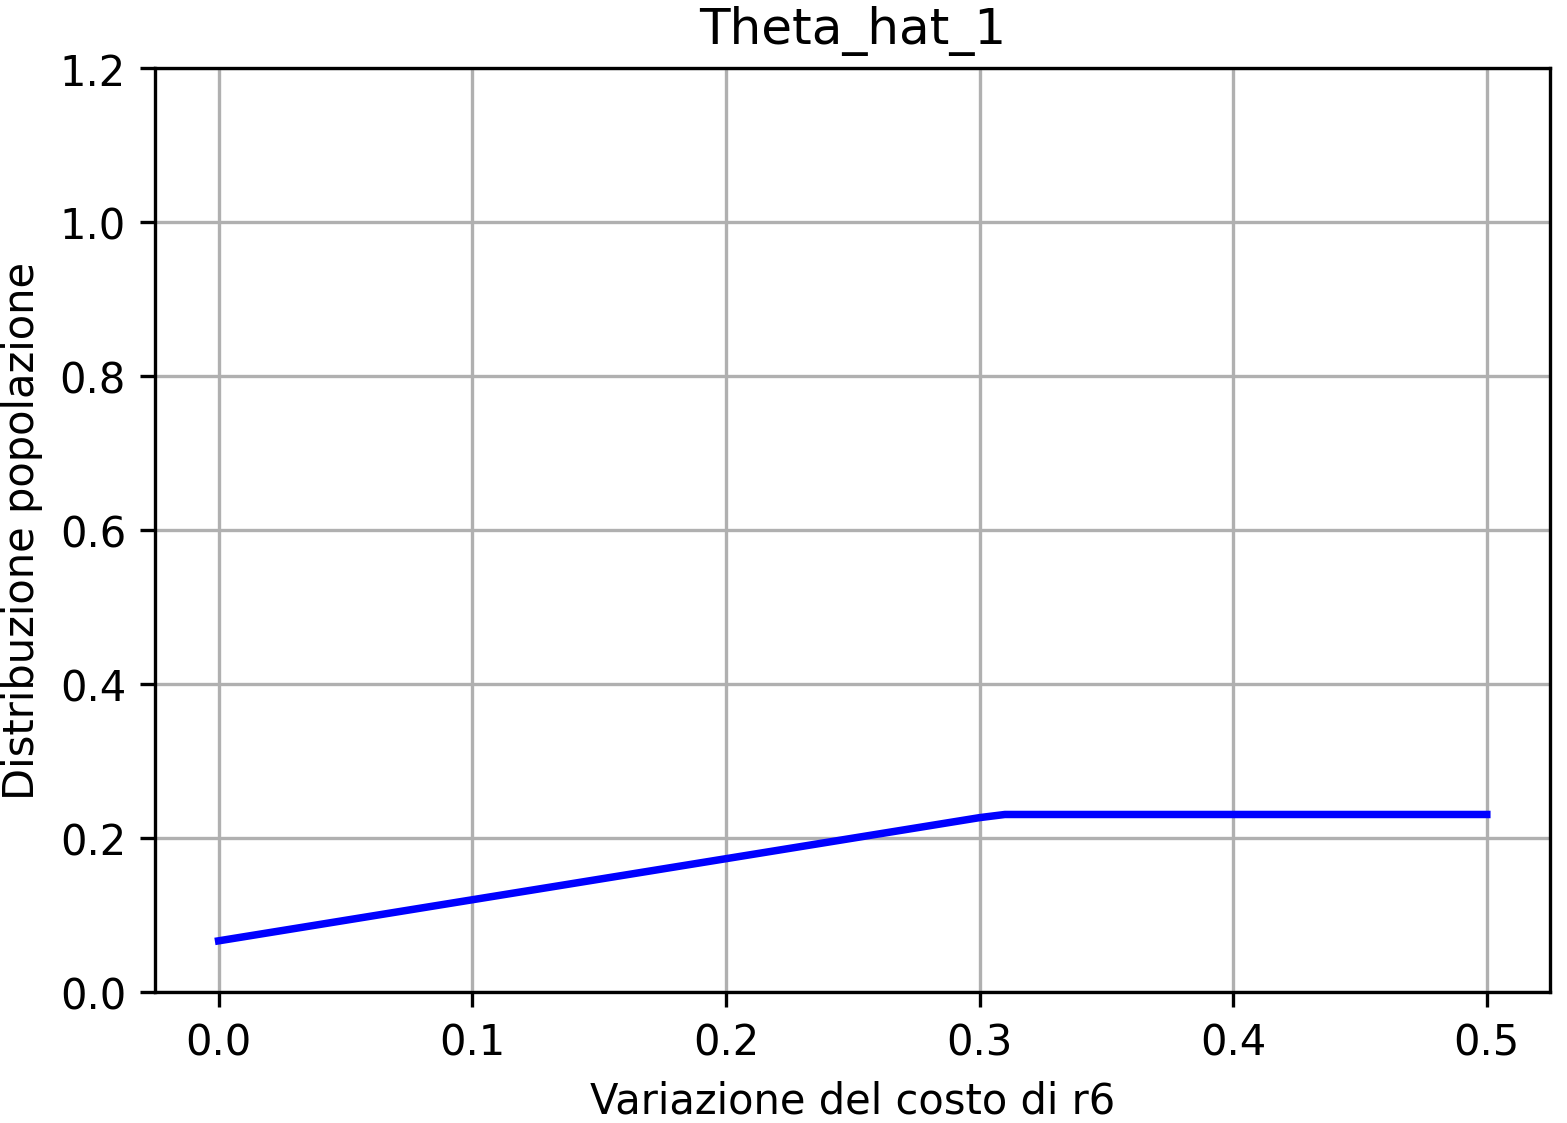
\includegraphics[width=0.42\textwidth]{figures/Es1/grafico_hat/hat_theta_1_Variazione_del_costo_di_r6.png}
        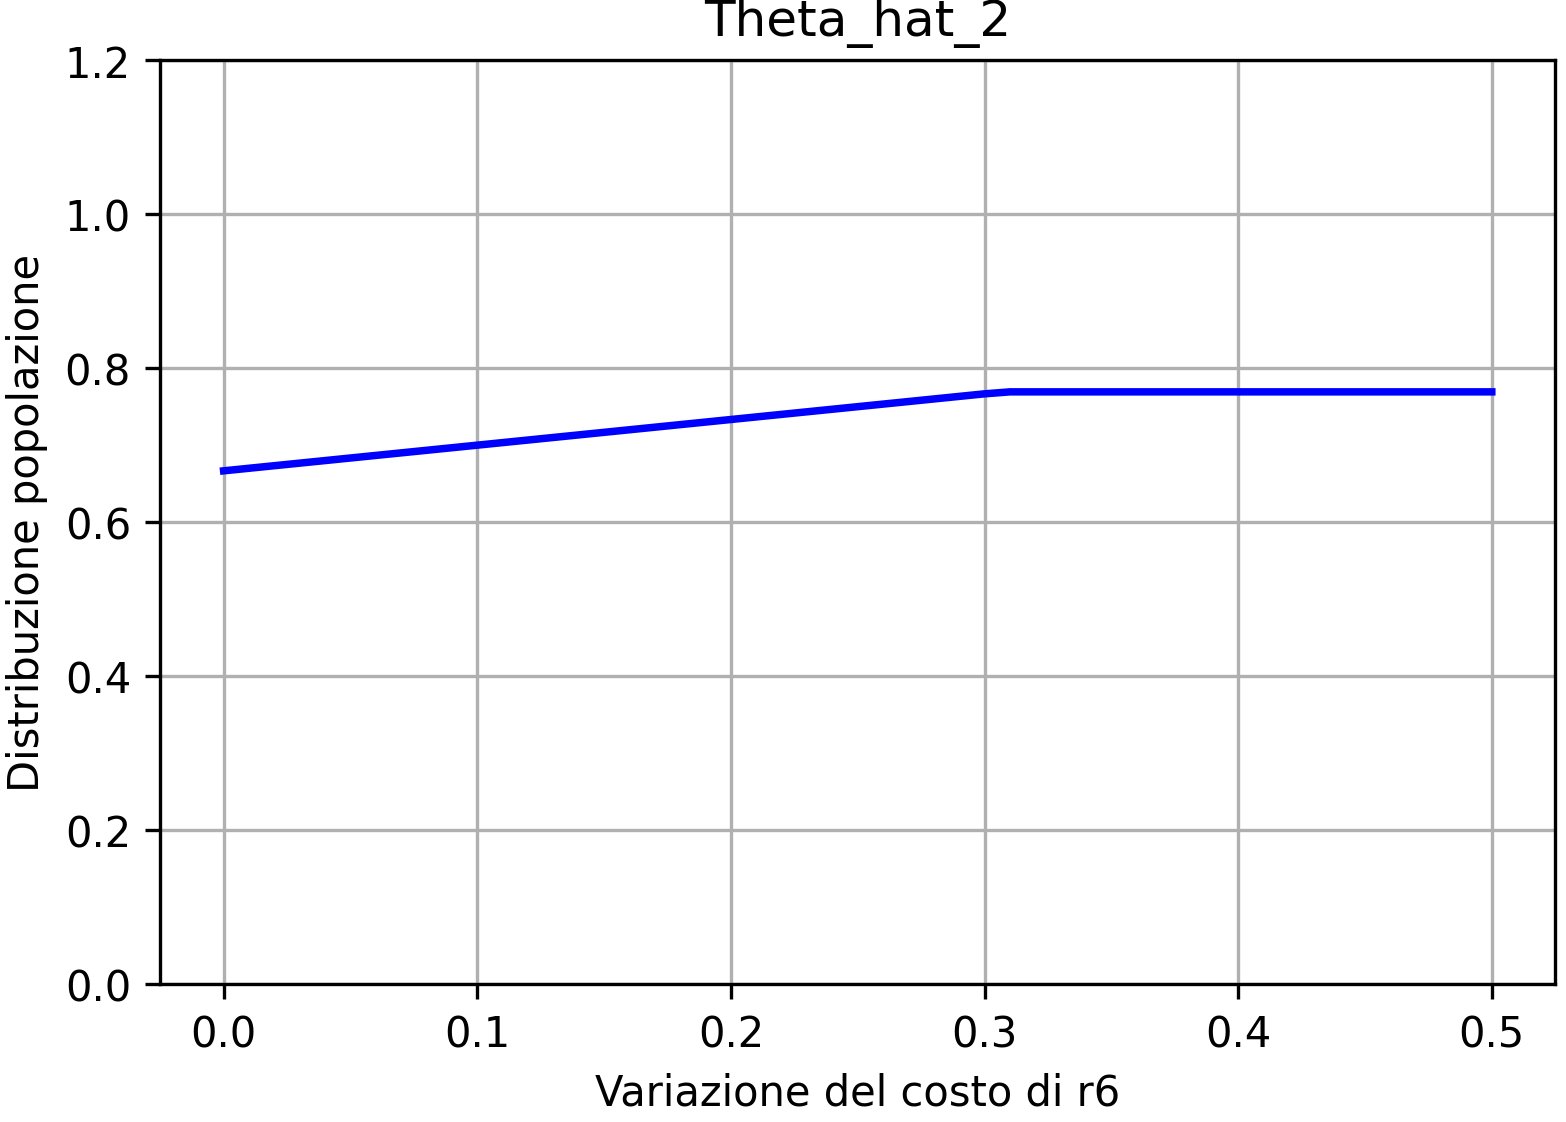
\includegraphics[width=0.42\textwidth]{figures/Es1/grafico_hat/hat_theta_2_Variazione_del_costo_di_r6.png}\\
        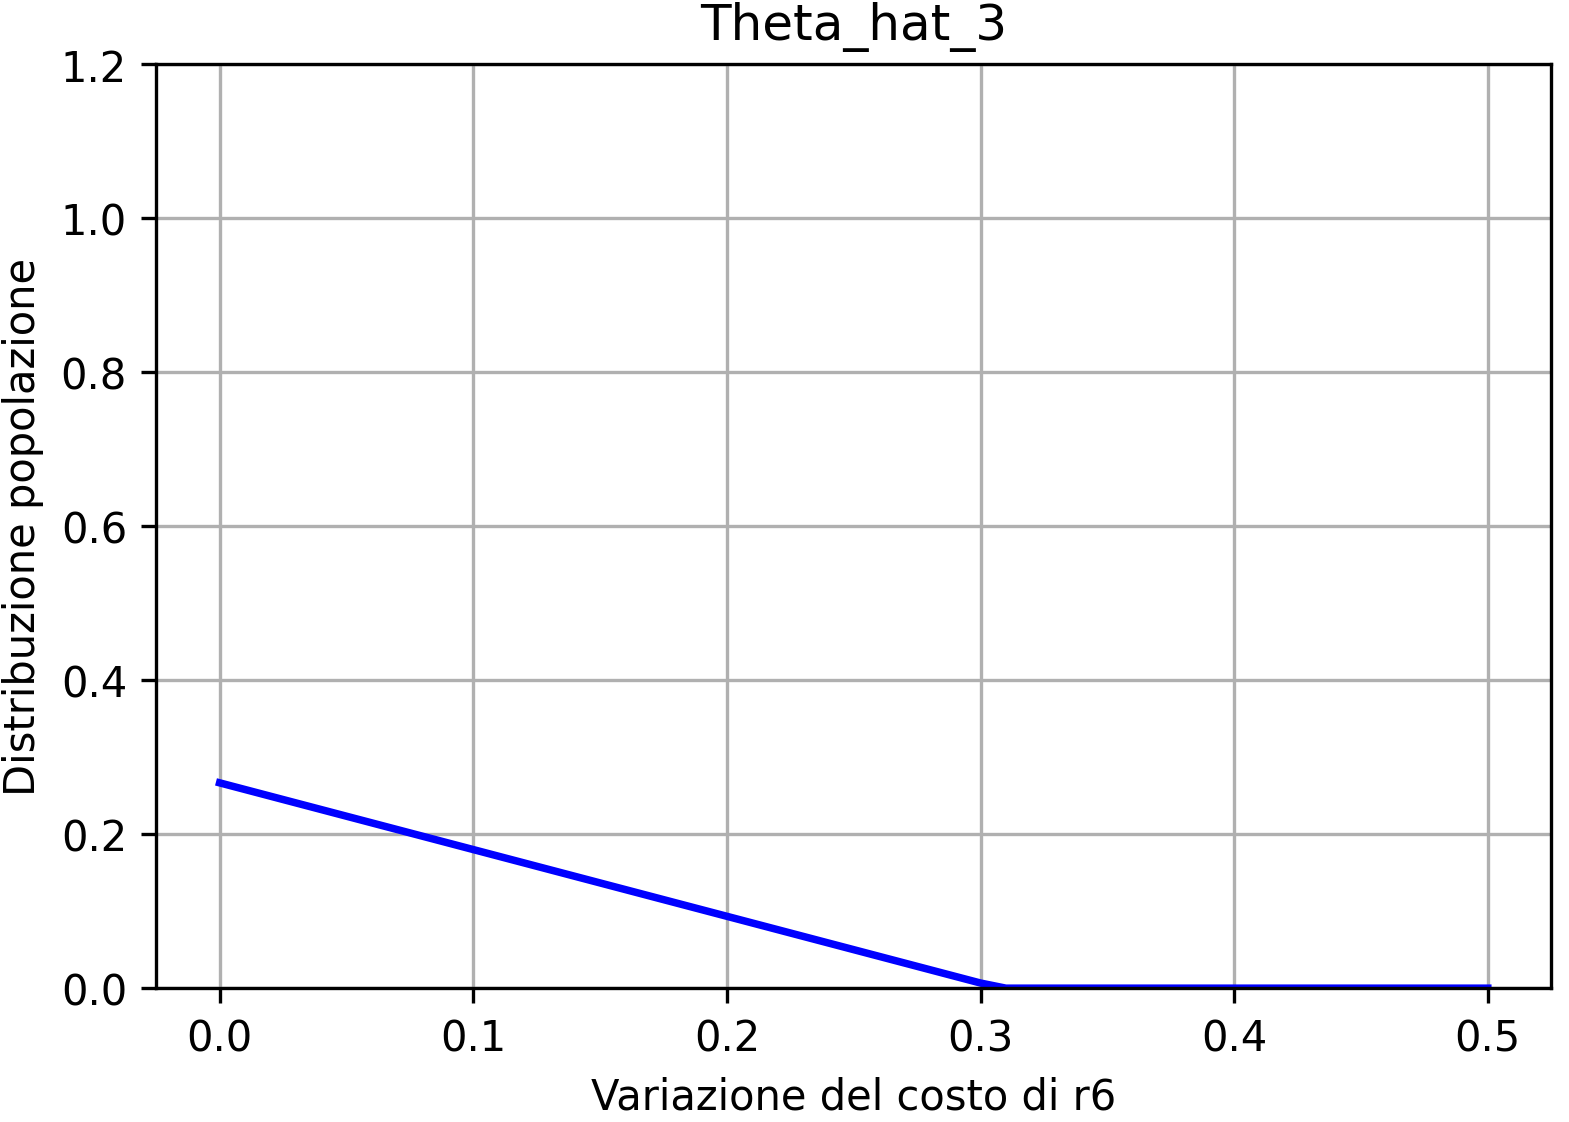
\includegraphics[width=0.42\textwidth]{figures/Es1/grafico_hat/hat_theta_3_Variazione_del_costo_di_r6.png}
        \end{center}
        \column{0.4\textwidth}
        \begin{center}
        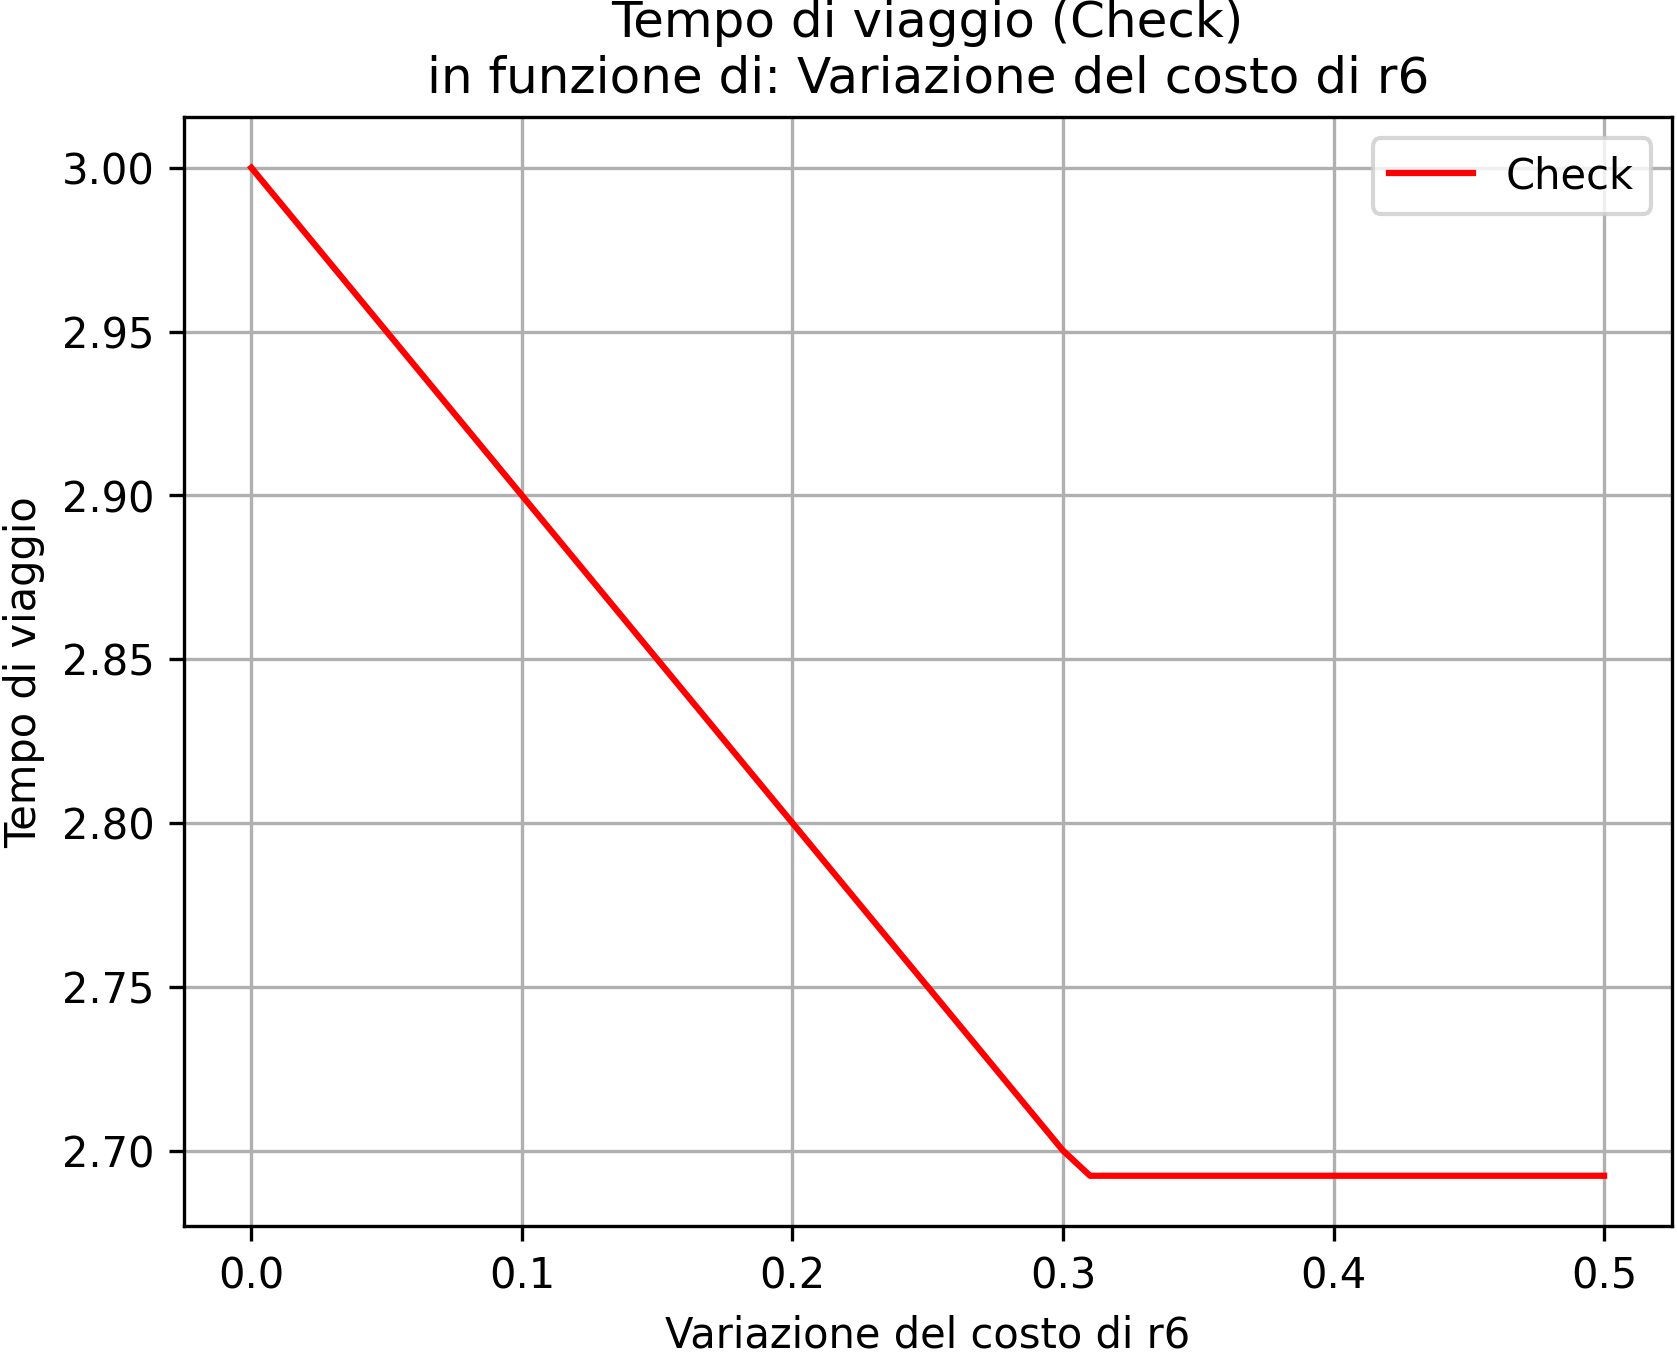
\includegraphics[width=1.0\textwidth]{figures/Es1/grafico_main_check_Variazione_del_costo_di_r6.png}
        \end{center}

    \end{columns}

    \begin{center}
    Aumentando il costo di $r_6$ per la popolazione \textit{hat} i tempi di viaggio per \textit{check} migliorano
    \end{center}

\end{frame}